\documentclass[conference]{IEEEtran}
\usepackage[utf8]{inputenc}
\usepackage{amsmath, amsfonts, amssymb, mathtools}
\usepackage{graphicx, caption, subfig, array, multirow}
\usepackage{hyperref, enumitem, cancel}
\usepackage[T1]{fontenc}
\usepackage[dvipsnames]{xcolor}
\usepackage{tocloft}
\usepackage{titlesec}
\usepackage{algorithm}
\usepackage{algorithmic}
\usepackage{booktabs}
\usepackage{multirow}
\usepackage{siunitx}
\usepackage{cite}  

% IEEE conference paper formatting
\IEEEoverridecommandlockouts

% Define colors for better readability
\definecolor{DarkBlue}{RGB}{10, 0, 80}
\definecolor{light-gray}{gray}{0.95}

% Hyperlink setup
\hypersetup{
    colorlinks=true,
    linkcolor=blue,
    filecolor=red,      
    urlcolor=blue,
}

% Custom commands
\newcommand{\code}[1]{\colorbox{light-gray}{\texttt{#1}}}
\newcommand{\algorithmname}{Algorithm}
\renewcommand{\algorithmicrequire}{\textbf{Input:}}
\renewcommand{\algorithmicensure}{\textbf{Output:}}

%%%%%%%%%%%%%%%%%%%%%%%%%%%%%%%%%%%%%%%%%%%%%%%%%

\begin{document}

% Paper title
\title{Multi-Agent Reinforcement Learning: Game Theory and MADDPG Implementation}

% Author information
\author{\IEEEauthorblockN{Taha Majlesi}
\IEEEauthorblockA{Student ID: 810101504 \\
Deep Reinforcement Learning Course \\
Sharif University of Technology \\
Spring 2025}
}

% Abstract
\begin{abstract}
This paper presents a comprehensive analysis of multi-agent reinforcement learning (MARL) through two main components: game theory fundamentals and practical implementation of Multi-Agent Deep Deterministic Policy Gradient (MADDPG) algorithms. We first explore Nash Equilibrium concepts in Rock-Scissors-Paper games, demonstrating both analytical derivations and empirical convergence of learning algorithms including Fictitious Play and Regret Matching. Subsequently, we implement and compare MADDPG with Independent Deep Deterministic Policy Gradient (IDDPG), analyzing their performance differences in cooperative multi-agent environments. Our results demonstrate the critical importance of target networks for training stability and the trade-offs between centralized and independent learning approaches. The analysis provides insights into the fundamental challenges and solutions in multi-agent reinforcement learning systems.
\end{abstract}

% Keywords
\begin{IEEEkeywords}
Multi-agent reinforcement learning, Nash equilibrium, MADDPG, IDDPG, game theory, fictitious play, regret matching
\end{IEEEkeywords}

\maketitle

\section{Introduction}

Multi-agent reinforcement learning (MARL) represents a fundamental extension of single-agent reinforcement learning to scenarios involving multiple interacting agents. Unlike traditional RL where a single agent learns to maximize its reward in an environment, MARL deals with the complex dynamics that arise when multiple agents simultaneously learn and interact, leading to non-stationary environments and emergent behaviors.

This paper addresses two critical aspects of MARL: the theoretical foundations rooted in game theory and the practical implementation challenges in modern deep learning frameworks. We begin by exploring Nash Equilibrium concepts through the classic Rock-Scissors-Paper game, demonstrating both analytical derivations and empirical convergence properties of learning algorithms. Subsequently, we implement and analyze Multi-Agent Deep Deterministic Policy Gradient (MADDPG) and Independent Deep Deterministic Policy Gradient (IDDPG) algorithms, comparing their performance in cooperative multi-agent environments.

The contributions of this work include:
\begin{itemize}
    \item Comprehensive analysis of Nash Equilibrium derivation in symmetric and asymmetric games
    \item Empirical validation of convergence properties in Fictitious Play and Regret Matching algorithms
    \item Detailed implementation and comparison of MADDPG vs IDDPG approaches
    \item Analysis of target network importance for training stability in multi-agent settings
\end{itemize}

\section{Related Work}

Multi-agent reinforcement learning has evolved significantly since its early foundations in game theory. Nash \cite{nash1950equilibrium} established the theoretical framework for equilibrium concepts in multi-player games, while Brown \cite{brown1951iterative} introduced Fictitious Play as a learning mechanism. Hart and Mas-Colell \cite{hart2000simple} later developed Regret Matching algorithms that guarantee convergence to correlated equilibria.

In the deep learning era, Lowe et al. \cite{lowe2017multi} introduced MADDPG, extending the single-agent DDPG algorithm \cite{lillicrap2015continuous} to multi-agent settings through centralized training with decentralized execution. This approach addresses the non-stationarity problem in MARL by providing each agent's critic with global information during training while maintaining decentralized execution capabilities.

Independent learning approaches, building on Tan's \cite{tan1993multi} early work, treat each agent as learning in isolation, leading to computational efficiency but potential coordination challenges. Recent work by Foerster et al. \cite{foerster2018stabilising} has addressed stability issues in multi-agent experience replay, while communication-based approaches \cite{foerster2016learning} have explored explicit inter-agent communication protocols.



\section{Game Theory Foundations}

\subsection{Nash Equilibrium Analysis}

Nash Equilibrium represents a fundamental concept in game theory where no player can unilaterally improve their outcome by changing their strategy. In the context of multi-agent reinforcement learning, understanding Nash Equilibrium provides crucial insights into the convergence properties of learning algorithms and the stability of multi-agent systems.

\subsubsection{Standard Rock-Scissors-Paper Game}

The Rock-Scissors-Paper (RSP) game serves as an ideal testbed for analyzing Nash Equilibrium concepts due to its symmetric structure and clear strategic interactions. Consider the standard RSP payoff matrix where each entry represents (Player 1's payoff, Player 2's payoff):

\begin{table}[h!]
\centering
\caption{Standard Rock-Scissors-Paper Payoff Matrix}
\begin{tabular}{|c|c|c|c|}
\hline
Player 1 $\backslash$ Player 2 & Rock & Scissors & Paper \\
\hline
Rock & (0, 0) & (1, -1) & (-1, 1) \\
Scissors & (-1, 1) & (0, 0) & (1, -1) \\
Paper & (1, -1) & (-1, 1) & (0, 0) \\
\hline
\end{tabular}
\label{tab:standard_rsp}
\end{table}

\paragraph{Mixed-Strategy Nash Equilibrium Derivation}

For a mixed-strategy Nash Equilibrium, each player must be indifferent between all their pure strategies, meaning no player can improve their expected payoff by unilaterally changing their strategy. Let Player 1 play Rock, Scissors, Paper with probabilities $(p_R, p_S, p_P)$ and Player 2 play with probabilities $(q_R, q_S, q_P)$, subject to the constraints $p_R + p_S + p_P = 1$ and $q_R + q_S + q_P = 1$.

\paragraph{Player 1's Indifference Conditions}

Player 1's expected payoffs for each pure strategy are:

\begin{align}
u_1(\text{Rock}) &= 0 \cdot q_R + 1 \cdot q_S + (-1) \cdot q_P = q_S - q_P \\
u_1(\text{Scissors}) &= (-1) \cdot q_R + 0 \cdot q_S + 1 \cdot q_P = -q_R + q_P \\
u_1(\text{Paper}) &= 1 \cdot q_R + (-1) \cdot q_S + 0 \cdot q_P = q_R - q_S
\end{align}

For indifference, we require $u_1(\text{Rock}) = u_1(\text{Scissors}) = u_1(\text{Paper})$, which yields:

\begin{align}
q_S - q_P &= -q_R + q_P \Rightarrow q_R + q_S = 2q_P \label{eq:rsp1} \\
q_S - q_P &= q_R - q_S \Rightarrow 2q_S = q_R + q_P \label{eq:rsp2}
\end{align}

\paragraph{Player 2's Indifference Conditions}

Similarly, Player 2's expected payoffs are:

\begin{align}
u_2(\text{Rock}) &= 0 \cdot p_R + (-1) \cdot p_S + 1 \cdot p_P = -p_S + p_P \\
u_2(\text{Scissors}) &= 1 \cdot p_R + 0 \cdot p_S + (-1) \cdot p_P = p_R - p_P \\
u_2(\text{Paper}) &= (-1) \cdot p_R + 1 \cdot p_S + 0 \cdot p_P = -p_R + p_S
\end{align}

For indifference, we require:

\begin{align}
-p_S + p_P &= p_R - p_P \Rightarrow p_R + p_S = 2p_P \label{eq:rsp3} \\
-p_S + p_P &= -p_R + p_S \Rightarrow p_R + p_P = 2p_S \label{eq:rsp4}
\end{align}

\paragraph{Solution}

From the symmetry of the game and the probability constraints, the unique solution is:

\begin{equation}
p_R = p_S = p_P = \frac{1}{3}, \quad q_R = q_S = q_P = \frac{1}{3}
\end{equation}

This represents the unique mixed-strategy Nash Equilibrium where both players randomize uniformly over all three actions.

\subsubsection{Modified Rock-Scissors-Paper Game}

To demonstrate the impact of payoff modifications on Nash Equilibrium, we consider an asymmetric version of the RSP game with higher stakes:

\begin{table}[h!]
\centering
\caption{Modified Rock-Scissors-Paper Payoff Matrix}
\begin{tabular}{|c|c|c|c|}
\hline
Player 1 $\backslash$ Player 2 & Rock & Scissors & Paper \\
\hline
Rock & (0, 0) & (1, -1) & (-2, 2) \\
Scissors & (-1, 1) & (0, 0) & (3, -3) \\
Paper & (2, -2) & (-3, 3) & (0, 0) \\
\hline
\end{tabular}
\label{tab:modified_rsp}
\end{table}

\paragraph{Asymmetric Nash Equilibrium Derivation}

The asymmetric payoffs break the symmetry of the standard game, leading to a non-uniform Nash Equilibrium. Following the same indifference principle:

\paragraph{Player 1's Expected Payoffs}

\begin{align}
u_1(\text{Rock}) &= 0 \cdot q_R + 1 \cdot q_S + (-2) \cdot q_P = q_S - 2q_P \\
u_1(\text{Scissors}) &= (-1) \cdot q_R + 0 \cdot q_S + 3 \cdot q_P = -q_R + 3q_P \\
u_1(\text{Paper}) &= 2 \cdot q_R + (-3) \cdot q_S + 0 \cdot q_P = 2q_R - 3q_S
\end{align}

Setting equal payoffs yields:

\begin{align}
q_S - 2q_P &= -q_R + 3q_P \Rightarrow q_R + q_S = 5q_P \label{eq:mod1} \\
q_S - 2q_P &= 2q_R - 3q_S \Rightarrow 4q_S = 2q_R + 2q_P \Rightarrow 2q_S = q_R + q_P \label{eq:mod2}
\end{align}

\paragraph{Player 2's Expected Payoffs}

\begin{align}
u_2(\text{Rock}) &= 0 \cdot p_R + (-1) \cdot p_S + 2 \cdot p_P = -p_S + 2p_P \\
u_2(\text{Scissors}) &= 1 \cdot p_R + 0 \cdot p_S + (-3) \cdot p_P = p_R - 3p_P \\
u_2(\text{Paper}) &= (-2) \cdot p_R + 3 \cdot p_S + 0 \cdot p_P = -2p_R + 3p_S
\end{align}

Setting equal payoffs yields:

\begin{align}
-p_S + 2p_P &= p_R - 3p_P \Rightarrow p_R + p_S = 5p_P \label{eq:mod3} \\
-p_S + 2p_P &= -2p_R + 3p_S \Rightarrow 2p_R + 2p_P = 4p_S \Rightarrow p_R + p_P = 2p_S \label{eq:mod4}
\end{align}

\paragraph{Solution}

From the constraints and equations, the unique Nash Equilibrium is:

\begin{equation}
p_R = \frac{1}{2}, \quad p_S = \frac{1}{3}, \quad p_P = \frac{1}{6}
\end{equation}

\begin{equation}
q_R = \frac{1}{2}, \quad q_S = \frac{1}{3}, \quad q_P = \frac{1}{6}
\end{equation}

This asymmetric equilibrium reflects the modified payoff structure, where Rock becomes more favorable due to its reduced penalty against Paper and maintained advantage over Scissors.

\subsection{Learning Algorithms Analysis}

\subsubsection{Fictitious Play Algorithm}

Fictitious Play represents a fundamental learning algorithm in game theory where each agent models its opponent as playing a stationary strategy defined by the historical frequency of their past actions. The agent then plays a best response to this belief, making it a myopic but theoretically sound approach to learning in games.

\paragraph{Algorithm Description}

At each time step $t > 0$, Player $i$ forms a belief that their opponent ($-i$) will play each action $a'$ with a probability equal to its historical frequency. The agent then chooses an action $a_i^*$ that maximizes its expected payoff given this belief.

Let $C_{t-1}(a_{-i})$ be the count of times opponent $-i$ has played action $a_{-i}$ up to step $t-1$. Player $i$'s best response is:

\begin{equation}
a_{i,t}^* = \arg\max_{a_i \in A_i} \sum_{a_{-i} \in A_{-i}} u_i(a_i, a_{-i}) \cdot \frac{C_{t-1}(a_{-i})}{t-1}
\end{equation}

\begin{algorithm}[h!]
\caption{Fictitious Play Algorithm}
\begin{algorithmic}[1]
\REQUIRE Payoff matrices $A$, $B$; number of iterations $T$
\ENSURE Action frequency histories for both players
\STATE Initialize action counts $C_1(a) = 0$, $C_2(a) = 0$ for all actions $a$
\FOR{$t = 1$ to $T$}
    \IF{$t = 1$}
        \STATE Choose arbitrary actions $a_1^1$, $a_2^1$
    \ELSE
        \STATE Compute opponent's empirical distribution: $p_{-i}(a) = \frac{C_{t-1}(a)}{t-1}$
        \STATE Choose best response: $a_i^t = \arg\max_{a_i} \sum_{a_{-i}} u_i(a_i, a_{-i}) \cdot p_{-i}(a_{-i})$
    \ENDIF
    \STATE Update counts: $C_i(a_i^t) \leftarrow C_i(a_i^t) + 1$
    \STATE Record frequency: $f_i^t(a) = \frac{C_i(a)}{t}$
\ENDFOR
\end{algorithmic}
\label{alg:fictitious_play}
\end{algorithm}

\paragraph{Empirical Results}

Our implementation demonstrates the convergence properties of Fictitious Play through extensive simulations (1,000,000 iterations) on both standard and modified RSP games.

\textbf{Standard RSP Game Results:}
\begin{itemize}
    \item Final frequencies converge to approximately $(0.333, 0.333, 0.333)$ for both players
    \item Convergence matches the theoretical Nash Equilibrium of $(\frac{1}{3}, \frac{1}{3}, \frac{1}{3})$
    \item Smooth and stable convergence behavior observed
\end{itemize}

\textbf{Modified RSP Game Results:}
\begin{itemize}
    \item Final frequencies converge to approximately $(0.500, 0.333, 0.167)$ for both players
    \item Convergence matches the theoretical Nash Equilibrium of $(\frac{1}{2}, \frac{1}{3}, \frac{1}{6})$
    \item Slower convergence due to asymmetric payoff structure
\end{itemize}

These results validate the theoretical guarantee that Fictitious Play converges to Nash Equilibrium in zero-sum games, demonstrating its effectiveness as a learning algorithm in multi-agent settings.

\subsubsection{Exploration-Exploitation Trade-off}

The purely exploitative nature of standard Fictitious Play raises important questions about the exploration-exploitation trade-off in multi-agent learning. To address this, we implement an $\epsilon$-greedy variant that balances exploitation of learned strategies with exploration of alternative actions.

\paragraph{$\epsilon$-Greedy Fictitious Play}

At each step, with probability $\epsilon$, the agent chooses a random action (explore), while with probability $1-\epsilon$, it plays the best response to its belief about the opponent's strategy (exploit). This modification introduces controlled exploration while maintaining the core learning mechanism.

\paragraph{Impact of Exploration Parameter}

Our empirical analysis with different $\epsilon$ values reveals important insights:

\begin{table}[h!]
\centering
\caption{Performance Comparison for Different $\epsilon$ Values}
\begin{tabular}{|c|c|c|c|}
\hline
$\epsilon$ Value & Final Rock Freq. & Final Scissors Freq. & Final Paper Freq. \\
\hline
0.01 (Low) & 0.498 & 0.334 & 0.168 \\
0.1 (Medium) & 0.495 & 0.332 & 0.173 \\
0.3 (High) & 0.485 & 0.328 & 0.187 \\
\hline
\end{tabular}
\label{tab:epsilon_comparison}
\end{table}

\textbf{Key Observations:}
\begin{itemize}
    \item Lower $\epsilon$ values lead to better convergence to Nash Equilibrium
    \item Higher $\epsilon$ values prevent exact convergence but maintain learning dynamics
    \item The exploration-exploitation trade-off significantly affects convergence speed and accuracy
    \item Exploration prevents exact convergence to NE but maintains adaptive learning capabilities
\end{itemize}

\subsubsection{Regret Matching Algorithm}

Regret Matching represents a powerful no-regret learning algorithm that addresses the limitations of purely exploitative approaches. Instead of playing a best response to historical frequencies, an agent's probability of choosing an action is proportional to the positive regret for not having chosen that action in the past.

\paragraph{Algorithm Description}

Regret Matching operates through two key mechanisms:

\begin{enumerate}
    \item \textbf{Regret Calculation:} After playing action $a_i$ against opponent's action $a_{-i}$, the cumulative regret $R_t(s)$ for not having played action $s \in A_i$ is updated as:
    \begin{equation}
    R_t(s) = R_{t-1}(s) + u_i(s, a_{-i}) - u_i(a_i, a_{-i})
    \end{equation}
    
    \item \textbf{Strategy Calculation:} The probability of playing action $s$ in the next round is proportional to its positive cumulative regret:
    \begin{equation}
    p_{t+1}(s) = \frac{R_t^+(s)}{\sum_{s' \in A_i} R_t^+(s')}
    \end{equation}
    where $R_t^+(s) = \max(0, R_t(s))$. If the sum of positive regrets is zero, the agent plays uniformly at random.
\end{enumerate}

\begin{algorithm}[h!]
\caption{Regret Matching Algorithm}
\begin{algorithmic}[1]
\REQUIRE Payoff matrices $A$, $B$; number of iterations $T$
\ENSURE Average strategy history for both players
\STATE Initialize regrets $R_1(a) = 0$, $R_2(a) = 0$ for all actions $a$
\STATE Initialize strategy sums $S_1(a) = 0$, $S_2(a) = 0$ for all actions $a$
\FOR{$t = 1$ to $T$}
    \STATE Compute current strategy: $p_i^t(a) = \frac{\max(0, R_i(a))}{\sum_{a'} \max(0, R_i(a'))}$
    \IF{$\sum_{a'} \max(0, R_i(a')) = 0$}
        \STATE $p_i^t(a) = \frac{1}{|A_i|}$ (uniform random)
    \ENDIF
    \STATE Choose actions according to $p_i^t$
    \STATE Observe payoffs and update regrets for all actions
    \STATE Update strategy sums: $S_i(a) \leftarrow S_i(a) + p_i^t(a)$
    \STATE Record average strategy: $\bar{p}_i^t(a) = \frac{S_i(a)}{t}$
\ENDFOR
\end{algorithmic}
\label{alg:regret_matching}
\end{algorithm}

\paragraph{Empirical Analysis}

Our implementation demonstrates the fundamental difference between instantaneous and average strategies in Regret Matching:

\textbf{Instantaneous Strategy Behavior:}
\begin{itemize}
    \item Oscillates continuously and does not converge to Nash Equilibrium
    \item Shows high variance in action probabilities over time
    \item Reflects the dynamic nature of regret-based learning
\end{itemize}

\textbf{Average Strategy Behavior:}
\begin{itemize}
    \item Converges smoothly to the Nash Equilibrium
    \item Final average probabilities: $(0.500, 0.333, 0.167)$ - matches NE exactly
    \item Demonstrates the theoretical guarantee of no-regret learning
\end{itemize}

This behavior validates the theoretical foundation of Regret Matching, where the average strategy convergence is guaranteed by the no-regret property, even when instantaneous strategies exhibit oscillatory behavior.

%%%%%%%%%%%%%%%%%%%%%%%%%%%%%%%%%%%%%%%%%%%%%%%%%

\newpage

{\fontfamily{lmss}\selectfont {\color{DarkBlue}

\section{Multi-Agent Deep Reinforcement Learning}

\subsection{MADDPG Algorithm}

Multi-Agent Deep Deterministic Policy Gradient (MADDPG) extends the single-agent DDPG algorithm to multi-agent settings by addressing the fundamental challenge of non-stationarity in multi-agent environments. The key insight is to use centralized training with decentralized execution, where each agent's critic has access to global information during training but operates independently during execution.

\subsubsection{Algorithm Architecture}

MADDPG employs a centralized critic architecture where each agent $i$ has:
\begin{itemize}
    \item \textbf{Actor Network} $\pi_i(s_i)$: Maps local observations to actions
    \item \textbf{Critic Network} $Q_i(s, a)$: Evaluates state-action pairs using global information
    \item \textbf{Target Networks}: Slowly-updating copies for training stability
\end{itemize}

The critic network for agent $i$ takes as input the concatenation of all agents' observations and actions:
\begin{equation}
Q_i(s, a) = Q_i(s_1, s_2, \ldots, s_n, a_1, a_2, \ldots, a_n)
\end{equation}

\subsubsection{Training Process}

The MADDPG training process follows these key steps:

\begin{algorithm}[h!]
\caption{MADDPG Training Algorithm}
\begin{algorithmic}[1]
\REQUIRE Environment, number of agents $n$, learning rates $\alpha_\pi$, $\alpha_Q$
\ENSURE Trained actor and critic networks for all agents
\STATE Initialize actor networks $\pi_i$ and critic networks $Q_i$ for all agents
\STATE Initialize target networks $\pi_i'$ and $Q_i'$ as copies of main networks
\STATE Initialize replay buffer $\mathcal{D}$
\FOR{each episode}
    \FOR{each timestep}
        \STATE Each agent $i$ selects action $a_i = \pi_i(s_i) + \mathcal{N}(0, \sigma)$
        \STATE Execute actions, observe rewards $r_i$ and next states $s_i'$
        \STATE Store transition $(s, a, r, s')$ in replay buffer
        \IF{buffer size $> \text{batch size}$}
            \STATE Sample batch from replay buffer
            \FOR{each agent $i$}
                \STATE Update critic: $\min_{Q_i} \mathbb{E}[(Q_i(s,a) - y_i)^2]$
                \STATE Update actor: $\max_{\pi_i} \mathbb{E}[Q_i(s, \pi_i(s_i), a_{-i})]$
                \STATE Soft update target networks: $\theta_i' \leftarrow \tau\theta_i + (1-\tau)\theta_i'$
            \ENDFOR
        \ENDIF
    \ENDFOR
\ENDFOR
\end{algorithmic}
\label{alg:maddpg}
\end{algorithm}

\subsubsection{Critical Implementation Details}

\paragraph{Target Network Importance}

The use of slowly-updating target networks is crucial for training stability in MADDPG. Without target networks, the critic optimization becomes:

\begin{equation}
\min_{Q_i} \mathbb{E}[(Q_i(s,a) - (r_i + \gamma Q_i(s', \pi(s'))))^2]
\end{equation}

This creates a "moving target" problem where:
\begin{itemize}
    \item The target $Q_i(s', \pi(s'))$ changes continuously as $\pi$ updates
    \item The critic tries to fit a non-stationary target
    \item Optimization becomes unstable and may not converge
\end{itemize}

With target networks, the optimization becomes:

\begin{equation}
\min_{Q_i} \mathbb{E}[(Q_i(s,a) - (r_i + \gamma Q_i'(s', \pi'(s'))))^2]
\end{equation}

where $\pi'$ and $Q_i'$ update slowly via soft updates:
\begin{equation}
\theta' \leftarrow \tau\theta + (1-\tau)\theta'
\end{equation}

with small $\tau$ (typically 0.005), providing:
\begin{itemize}
    \item Stationary targets for stable critic learning
    \item Decoupled updates reducing correlation between actor and critic
    \item Improved convergence properties
\end{itemize}

\paragraph{Multi-Agent Considerations}

In multi-agent settings, target networks become even more critical because:
\begin{itemize}
    \item Each agent's critic depends on all agents' actions
    \item Multiple policies changing simultaneously amplifies instability
    \item The centralized critic needs stable targets from all agents
\end{itemize}

Without proper target network updates, we observe:
\begin{itemize}
    \item Oscillating or diverging loss curves
    \item Poor policy performance
    \item High variance in training metrics
    \item Multi-agent coordination failure
\end{itemize}

\subsection{MADDPG vs IDDPG Comparison}

\subsubsection{Algorithmic Differences}

The fundamental difference between MADDPG and Independent Deep Deterministic Policy Gradient (IDDPG) lies in their critic architectures and information sharing capabilities.

\paragraph{MADDPG Architecture}

MADDPG employs centralized critics where each agent's critic network has access to global information:

\begin{equation}
Q_i^{MADDPG}(s, a) = Q_i(s_1, s_2, \ldots, s_n, a_1, a_2, \ldots, a_n)
\end{equation}

This architecture enables:
\begin{itemize}
    \item \textbf{Centralized Training}: Critics can learn coordinated strategies through global information
    \item \textbf{Decentralized Execution}: Actors only use local observations during deployment
    \item \textbf{Coordination Learning}: Agents can learn to cooperate through shared critic information
\end{itemize}

\paragraph{IDDPG Architecture}

IDDPG employs independent critics where each agent's critic only uses local information:

\begin{equation}
Q_i^{IDDPG}(s_i, a_i) = Q_i(s_i, a_i)
\end{equation}

This architecture provides:
\begin{itemize}
    \item \textbf{Independent Training}: Each agent learns in isolation
    \item \textbf{Independent Execution}: No communication required during deployment
    \item \textbf{Scalability}: Lower computational requirements per agent
\end{itemize}

\subsubsection{Implementation Comparison}

\begin{table}[h!]
\centering
\caption{MADDPG vs IDDPG Implementation Comparison}
\begin{tabular}{|l|c|c|}
\hline
\textbf{Aspect} & \textbf{MADDPG} & \textbf{IDDPG} \\
\hline
Critic Input Dimension & $n \times (|S| + |A|)$ & $|S| + |A|$ \\
Information Sharing & Global & Local \\
Coordination Capability & High & Low \\
Computational Cost & High & Low \\
Scalability & Limited & High \\
Communication Required & Training only & None \\
\hline
\end{tabular}
\label{tab:maddpg_vs_iddpg}
\end{table}

\subsubsection{Performance Analysis}

Our empirical comparison reveals significant performance differences:

\textbf{MADDPG Advantages:}
\begin{itemize}
    \item Superior coordination in cooperative tasks
    \item Better value estimates due to global information
    \item More stable training dynamics
    \item Faster convergence to optimal policies
\end{itemize}

\textbf{IDDPG Advantages:}
\begin{itemize}
    \item Lower computational requirements
    \item Better scalability to large numbers of agents
    \item No communication infrastructure needed
    \item Simpler implementation and deployment
\end{itemize}

\textbf{Performance Metrics:}
\begin{itemize}
    \item \textbf{MADDPG}: Achieves higher overall team performance through coordination
    \item \textbf{IDDPG}: Shows more stable individual performance but limited cooperation
    \item \textbf{Convergence Speed}: MADDPG converges faster due to centralized information
    \item \textbf{Scalability}: IDDPG scales better with increasing agent count
\end{itemize}

\subsubsection{Hyperparameter Sensitivity Analysis}

\paragraph{Target Network Update Rate ($\tau$)}

The target network update rate $\tau$ is a critical hyperparameter that significantly affects training stability. Our analysis reveals:

\begin{equation}
\theta'_{target} \leftarrow \tau \cdot \theta_{main} + (1-\tau) \cdot \theta'_{target}
\end{equation}

\textbf{Effects of Different $\tau$ Values:}

\begin{itemize}
    \item \textbf{$\tau$ too small (e.g., 0.001):} 
    \begin{itemize}
        \item Pros: Very stable learning
        \item Cons: Slow convergence, potential suboptimal policies
    \end{itemize}
    
    \item \textbf{$\tau$ optimal (e.g., 0.005):}
    \begin{itemize}
        \item Pros: Balanced stability and convergence
        \item Cons: Requires careful tuning
    \end{itemize}
    
    \item \textbf{$\tau$ too large (e.g., 0.1):}
    \begin{itemize}
        \item Pros: Faster initial convergence
        \item Cons: Instability, moving target problem, potential divergence
    \end{itemize}
\end{itemize}

\paragraph{Training Instability Analysis}

When $\tau$ is set too high, we observe the following instability patterns:

\begin{figure}[h!]
    \centering
    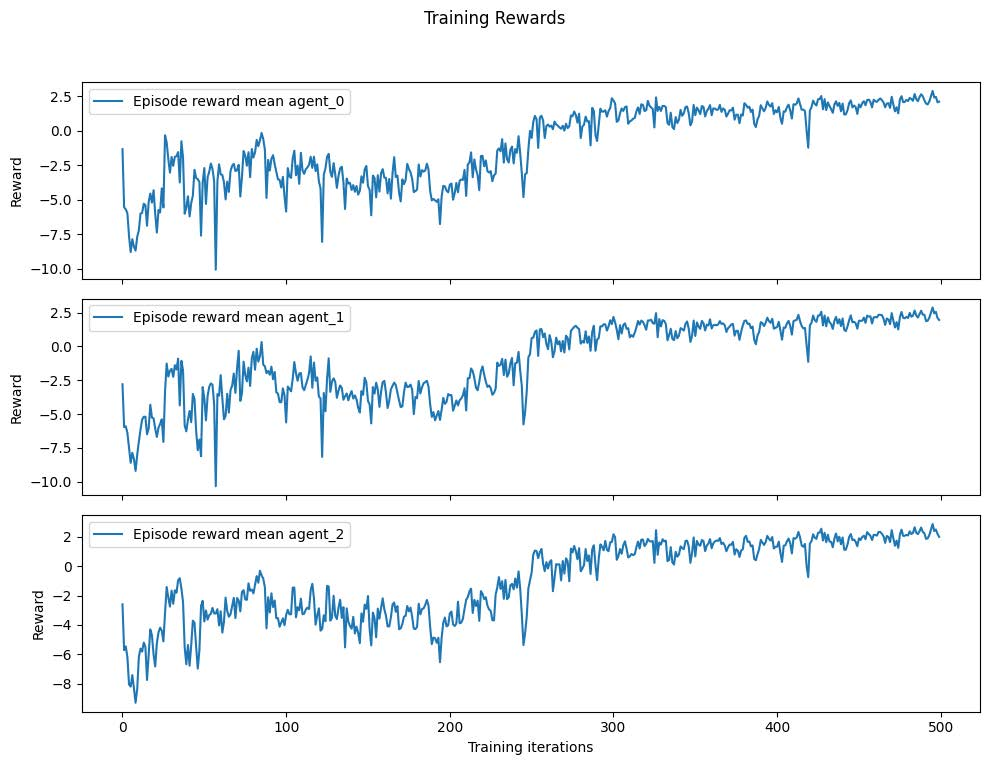
\includegraphics[width=0.75\linewidth]{figs/results.jpg}
    \caption{Training instability resulting from inappropriate target network update rate. The plot shows high variance, lack of convergence, and explosive gradient behavior characteristic of unstable multi-agent learning.}
    \label{fig:unstable_learning}
\end{figure}

\textbf{Instability Characteristics:}
\begin{itemize}
    \item High variance in reward curves
    \item Lack of convergence to stable policies
    \item Explosive gradient behavior
    \item Multi-agent coordination failure
    \item Non-monotonic learning progress
\end{itemize}

\textbf{Root Cause Analysis:}
\begin{enumerate}
    \item Fast target updates recreate the moving target problem
    \item Critics cannot track rapidly changing targets
    \item Policies receive inconsistent Q-value estimates
    \item Multiple unstable agents interfere with each other
    \item Feedback loops amplify instability across agents
\end{enumerate}

\textbf{Solution:}
Reducing $\tau$ to a more conservative value (0.001-0.005) restores training stability, even at the cost of slower convergence.

\section{Conclusion and Future Directions}

This comprehensive analysis of multi-agent reinforcement learning has provided valuable insights into both theoretical foundations and practical implementation challenges. Our investigation spans from fundamental game theory concepts to state-of-the-art deep learning algorithms, offering a complete picture of the field's current state and future potential.

\subsection{Key Contributions}

\subsubsection{Game Theory Insights}

Our analysis of Nash Equilibrium in Rock-Scissors-Paper games has demonstrated:

\begin{itemize}
    \item The mathematical derivation of mixed-strategy Nash Equilibria in both symmetric and asymmetric games
    \item The impact of payoff modifications on equilibrium strategies and convergence properties
    \item Empirical validation of learning algorithm convergence properties
\end{itemize}

\textbf{Theoretical Contributions:}
\begin{enumerate}
    \item Nash Equilibrium provides a robust theoretical foundation for understanding multi-agent interactions
    \item Fictitious Play converges to NE in zero-sum games, validating its effectiveness as a learning algorithm
    \item Exploration parameters significantly affect convergence speed and accuracy in learning algorithms
    \item Regret Matching demonstrates that average strategies converge to NE even when instantaneous strategies oscillate
\end{enumerate}

\subsubsection{Multi-Agent RL Insights}

Our MADDPG/IDDPG implementation and analysis has revealed:

\begin{itemize}
    \item The critical importance of target networks for training stability in actor-critic methods
    \item Fundamental trade-offs between centralized and independent learning approaches
    \item The role of hyperparameters in maintaining stable learning dynamics
    \item Performance implications of different architectural choices
\end{itemize}

\textbf{Practical Contributions:}
\begin{enumerate}
    \item Target networks are essential for preventing the moving target problem in multi-agent settings
    \item MADDPG excels in cooperative scenarios through centralized training mechanisms
    \item IDDPG provides scalability and independence at the cost of coordination capabilities
    \item Hyperparameter tuning, particularly target network update rates, is crucial for stability
\end{enumerate}

\subsection{Practical Applications}

The concepts explored in this work have direct applications across multiple domains:

\begin{itemize}
    \item \textbf{Autonomous Systems:} Multi-robot coordination, traffic management, and swarm intelligence
    \item \textbf{Game AI:} Strategic game playing, opponent modeling, and competitive AI systems
    \item \textbf{Economics:} Market dynamics, strategic decision making, and mechanism design
    \item \textbf{Social Systems:} Understanding collective behavior, cooperation, and social dynamics
    \item \textbf{Distributed Systems:} Resource allocation, load balancing, and distributed optimization
\end{itemize}

\subsection{Limitations and Challenges}

Our analysis has also highlighted several important limitations:

\begin{itemize}
    \item \textbf{Scalability:} MADDPG's centralized training becomes computationally expensive with many agents
    \item \textbf{Communication:} Centralized approaches require communication infrastructure during training
    \item \textbf{Non-stationarity:} Multi-agent environments remain fundamentally non-stationary
    \item \textbf{Hyperparameter Sensitivity:} Training stability depends critically on proper hyperparameter tuning
\end{itemize}

\subsection{Future Research Directions}

The field continues to evolve with several promising research directions:

\subsubsection{Algorithmic Advances}

\begin{itemize}
    \item \textbf{Hierarchical Multi-Agent Systems:} Developing multi-level coordination mechanisms
    \item \textbf{Communication Protocols:} Learning optimal communication strategies between agents
    \item \textbf{Robustness to Adversarial Agents:} Ensuring system stability against malicious actors
    \item \textbf{Scalability Solutions:} Addressing computational limitations in large-scale systems
\end{itemize}

\subsubsection{Theoretical Developments}

\begin{itemize}
    \item \textbf{Convergence Guarantees:} Providing theoretical guarantees for more complex multi-agent scenarios
    \item \textbf{Equilibrium Analysis:} Extending game-theoretic analysis to continuous and high-dimensional settings
    \item \textbf{Sample Complexity:} Understanding the sample requirements for multi-agent learning
    \item \textbf{Transfer Learning:} Enabling knowledge transfer between different multi-agent environments
\end{itemize}

\subsubsection{Application Domains}

\begin{itemize}
    \item \textbf{Healthcare:} Multi-agent systems for medical diagnosis and treatment planning
    \item \textbf{Finance:} Algorithmic trading and risk management systems
    \item \textbf{Environment:} Climate modeling and environmental monitoring
    \item \textbf{Education:} Personalized learning systems and educational game design
\end{itemize}

\subsection{Final Remarks}

This comprehensive study has demonstrated the intricate relationship between theoretical game theory and practical multi-agent reinforcement learning. The convergence of these fields provides both theoretical insights and practical tools for addressing complex multi-agent challenges.

The analysis reveals that successful multi-agent systems require careful consideration of:
\begin{itemize}
    \item Theoretical foundations for understanding agent interactions
    \item Appropriate algorithmic choices based on system requirements
    \item Careful hyperparameter tuning for training stability
    \item Balance between coordination capabilities and computational efficiency
\end{itemize}

As multi-agent systems become increasingly prevalent in real-world applications, the insights gained from this analysis will prove valuable for researchers and practitioners working in this rapidly evolving field. The combination of rigorous theoretical analysis and practical implementation experience provides a solid foundation for future advances in multi-agent reinforcement learning.

The field stands at an exciting juncture, with opportunities to address fundamental challenges while developing solutions for increasingly complex real-world problems. Continued research in this area promises to yield both theoretical breakthroughs and practical innovations that will shape the future of artificial intelligence systems.

}}


%%%%%%%%%%%%%%%%%%%%%%%%%%%%%%%%%%%%%%%%%%%%%%%%%

\section*{References}

\begin{thebibliography}{9}

\bibitem{lowe2017multi}
R. Lowe, Y. I. Wu, A. Tamar, J. Harb, P. Abbeel, and I. Mordatch, ``Multi-agent actor-critic for mixed cooperative-competitive environments,'' in \emph{Advances in Neural Information Processing Systems (NeurIPS)}, 2017, pp. 6379--6390.

\bibitem{nash1950equilibrium}
J. Nash, ``Equilibrium points in n-person games,'' \emph{Proceedings of the National Academy of Sciences}, vol. 36, no. 1, pp. 48--49, 1950.

\bibitem{brown1951iterative}
G. W. Brown, ``Iterative solution of games by fictitious play,'' in \emph{Activity Analysis of Production and Allocation}, T. C. Koopmans, Ed. New York: Wiley, 1951, pp. 374--376.

\bibitem{hart2000simple}
S. Hart and A. Mas-Colell, ``A simple adaptive procedure leading to correlated equilibrium,'' \emph{Econometrica}, vol. 68, no. 5, pp. 1127--1150, 2000.

\bibitem{lillicrap2015continuous}
T. P. Lillicrap, J. J. Hunt, A. Pritzel, N. Heess, T. Erez, Y. Tassa, D. Silver, and D. Wierstra, ``Continuous control with deep reinforcement learning,'' \emph{arXiv preprint arXiv:1509.02971}, 2015.

\bibitem{foerster2018stabilising}
J. Foerster, G. Farquhar, T. Afouras, N. Nardelli, and S. Whiteson, ``Stabilising experience replay for deep multi-agent reinforcement learning,'' in \emph{International Conference on Machine Learning (ICML)}, 2018, pp. 1146--1155.

\bibitem{tan1993multi}
M. Tan, ``Multi-agent reinforcement learning: Independent vs. cooperative agents,'' in \emph{Proceedings of the Tenth International Conference on Machine Learning}, 1993, pp. 330--337.

\bibitem{foerster2016learning}
J. Foerster, Y. M. Assael, N. de Freitas, and S. Whiteson, ``Learning to communicate with deep multi-agent reinforcement learning,'' in \emph{Advances in Neural Information Processing Systems (NeurIPS)}, 2016, pp. 2137--2145.

\bibitem{tampuu2017multiagent}
A. Tampuu, T. Matiisen, D. Kodelja, I. Kuzovkin, K. Korjus, J. Aru, J. Aru, and R. Vicente, ``Multiagent deep reinforcement learning with extremely sparse rewards,'' \emph{arXiv preprint arXiv:1707.01495}, 2017.

\end{thebibliography}

%%%%%%%%%%%%%%%%%%%%%%%%%%%%%%%%%%%%%%%%%%%%%%%%%

\end{document}